% ============================================================
%  Phase-Adaptive GHB Data Cache Prefetcher --- Beamer Slides
%  CS Computer System Architecture, IIT Tirupati 2026
%  CS25M111 (P. Gurudeep)  &  CS25M112 (Prince Kumar)
% ============================================================
\documentclass[aspectratio=169,t]{beamer}

% ---------- Encoding ----------------------------------------
\usepackage[utf8]{inputenc}
\usepackage[T1]{fontenc}

% ---------- Theme & Colours ---------------------------------
\usetheme{Madrid}
\usecolortheme{whale}
\useinnertheme{rectangles}

\definecolor{iitblue}{RGB}{0,51,102}
\definecolor{iitgold}{RGB}{204,153,0}
\definecolor{darkgreen}{RGB}{0,120,0}
\definecolor{darkred}{RGB}{180,0,0}

\setbeamercolor{palette primary}{bg=iitblue,fg=white}
\setbeamercolor{palette secondary}{bg=iitblue!80,fg=white}
\setbeamercolor{palette tertiary}{bg=iitblue!60,fg=white}
\setbeamercolor{palette quaternary}{bg=iitblue,fg=white}
\setbeamercolor{structure}{fg=iitblue}
\setbeamercolor{section in toc}{fg=iitblue}
\setbeamercolor{alerted text}{fg=iitgold}
\setbeamercolor{block title}{bg=iitblue,fg=white}
\setbeamercolor{block body}{bg=iitblue!8}
\setbeamercolor{block title alerted}{bg=darkred,fg=white}
\setbeamercolor{block body alerted}{bg=darkred!8}
\setbeamercolor{block title example}{bg=darkgreen,fg=white}
\setbeamercolor{block body example}{bg=darkgreen!8}

% ---------- Packages ----------------------------------------
\usepackage{booktabs}
\usepackage{multirow}
\usepackage{colortbl}
\usepackage{xcolor}
\usepackage{graphicx}
\usepackage{adjustbox}
\usepackage{tikz}
\usetikzlibrary{shapes.geometric,arrows.meta,positioning,fit,backgrounds,calc}
\usepackage{listings}
\usepackage{array}
\usepackage{pgfplots}
\pgfplotsset{compat=1.18}
\usepackage{amsmath}
\usepackage{pifont}

% ---------- Listings style ----------------------------------
\lstset{
  basicstyle=\ttfamily\tiny,
  keywordstyle=\color{iitblue}\bfseries,
  commentstyle=\color{gray},
  stringstyle=\color{darkgreen},
  backgroundcolor=\color{iitblue!5},
  frame=single,
  framerule=0.4pt,
  frameround=tttt,
  breaklines=true,
  numbers=left,
  numberstyle=\tiny\color{gray},
  xleftmargin=1.5em
}

% ---------- Title info -------------------------------------
\title[Phase-Adaptive GHB Prefetcher]{\textbf{Phase-Adaptive Global History Buffer}\\[2pt]\textbf{Data Cache Prefetcher}}
\subtitle{CS5830 --- Computer System Architecture}
\author[CS25M111 \& CS25M112]{
  \textbf{P. Gurudeep} (CS25M111)\quad\&\quad\textbf{Prince Kumar} (CS25M112)
}
\institute[IIT Tirupati]{
  Department of Computer Science \& Engineering\\
  Indian Institute of Technology Tirupati
}
\date{April 30, 2026}

% ---------- Helper commands --------------------------------
\newcommand{\good}[1]{\textcolor{darkgreen}{\textbf{#1}}}
\newcommand{\bad}[1]{\textcolor{darkred}{\textbf{#1}}}
\newcommand{\hl}[1]{\textcolor{iitgold}{\textbf{#1}}}

% ===========================================================
\begin{document}

% ── TITLE SLIDE ────────────────────────────────────────────
\begin{frame}[plain]
  \titlepage
  \vspace{-6pt}
  \begin{center}
    \small
    \texttt{github.com/gurudeepDev/ghb-prefetcher}
    \quad|\quad
    Paper: Nesbit \& Smith, \textit{IEEE MICRO} 2004
  \end{center}
\end{frame}

% ── OUTLINE ────────────────────────────────────────────────
\begin{frame}{Outline}
  \tableofcontents
\end{frame}

% ===========================================================
\section{Block Diagram \& Integration}
% ===========================================================
\begin{frame}[shrink=3]{Slide 2 --- GHB Structure \& Integration with Cache Hierarchy}
\begin{columns}[T]
\column{0.46\textwidth}
\begin{center}
  \textbf{\footnotesize Concept: History Table $\rightarrow$ GHB}
\end{center}
\vspace{-4pt}
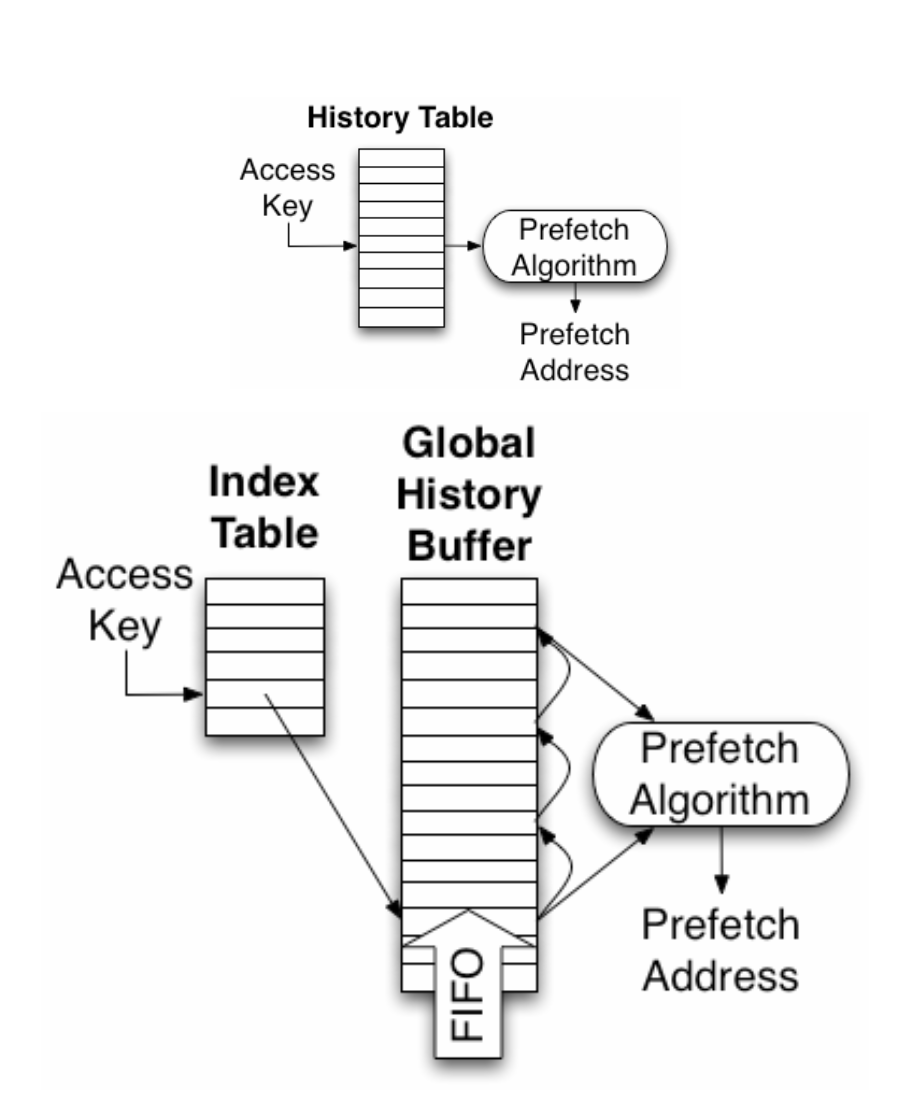
\includegraphics[width=\linewidth,height=0.62\textheight,keepaspectratio]{img/ghb-concept.png}

\column{0.26\textwidth}
\begin{center}
  \textbf{\footnotesize G/AC (PC-keyed)}\\[2pt]
  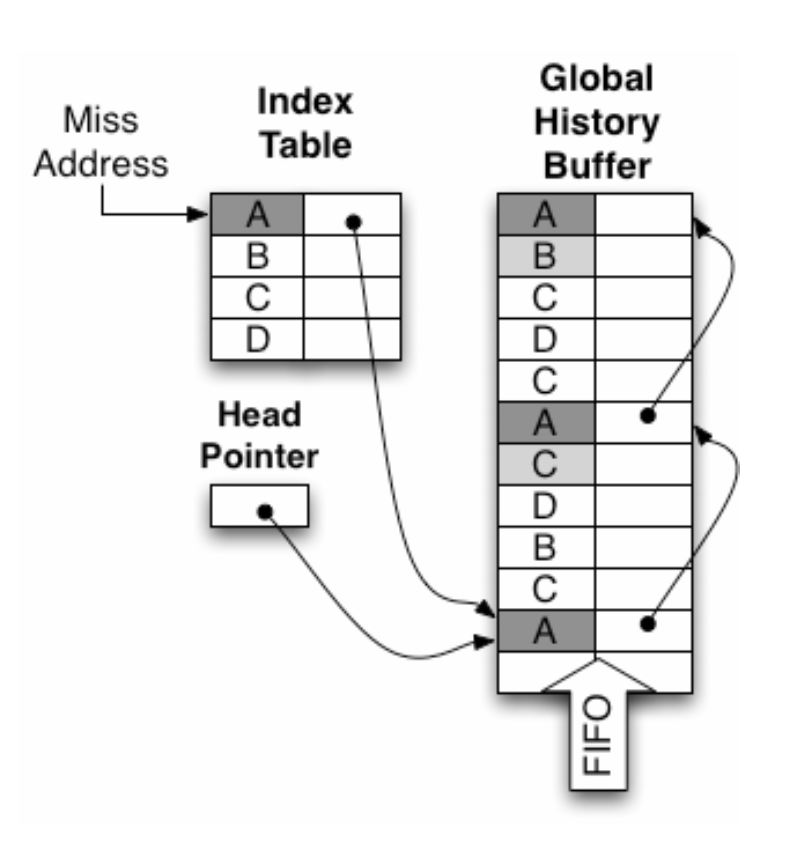
\includegraphics[width=\linewidth,keepaspectratio]{img/ghb-gac.png}
\end{center}

\column{0.26\textwidth}
\begin{exampleblock}{HW Overhead: \good{30 bits}}
\scriptsize
\begin{tabular}{@{}ll@{}}
\texttt{epoch\_ctr}   & 8 bits \\
\texttt{pf\_issued}   & 8 bits \\
\texttt{pf\_hits}     & 8 bits \\
\texttt{consec}       & 2 bits \\
\texttt{cur\_phase}   & 1 bit  \\
\texttt{degree}       & 3 bits \\
\end{tabular}
\end{exampleblock}
\begin{block}{Cache Hierarchy}
\scriptsize
\begin{tabular}{@{}ll@{}}
L1D  & 32\,KB, 4-cyc \\
L2   & 256\,KB, 10-cyc \\
LLC  & 2\,MB, 20-cyc \\
DRAM & 140 cycles \\
\end{tabular}
\end{block}
\end{columns}
\end{frame}

% ===========================================================
\section{Algorithm}
% ===========================================================
\begin{frame}{Slide 3 --- Algorithm: Phase-Adaptive GHB PC/DC}
\begin{columns}[T]
\column{0.52\textwidth}
\begin{block}{3-Step Algorithm}
\footnotesize
\textbf{[1] MONITOR} --- every $W=512$ accesses: count \texttt{pf\_hits/pf\_issued}\\[2pt]
\textbf{[2] CLASSIFY} epoch accuracy $a$:
\begin{itemize}\setlength\itemsep{0pt}\setlength\parsep{0pt}
  \item $a \ge 70\%$ $\Rightarrow$ \good{PREDICTABLE}
  \item $a \le 30\%$ $\Rightarrow$ \bad{IRREGULAR}
  \item $30\%\!<\!a\!<\!70\%$ $\Rightarrow$ dead zone (no change)
\end{itemize}
\textbf{[3] ACT} (hysteresis $N=2$): \good{PRED$\times$2}$\Rightarrow$\texttt{d=4};\ \bad{IRREG$\times$2}$\Rightarrow$\texttt{d=0}
\end{block}
\begin{alertblock}{Delta Prediction (GHB PC/DC core)}
\footnotesize
Walk chain $\rightarrow$ build delta sequence\\
Find last 2-delta pair $(d_0,d_1)$ $\rightarrow$ locate prev.\ match\\
Issue $\le$\texttt{degree} lines via \textit{pattern continuation}
\end{alertblock}

\column{0.46\textwidth}
\begin{center}
  \textbf{\footnotesize Phase Detection Flowchart}\\[3pt]
  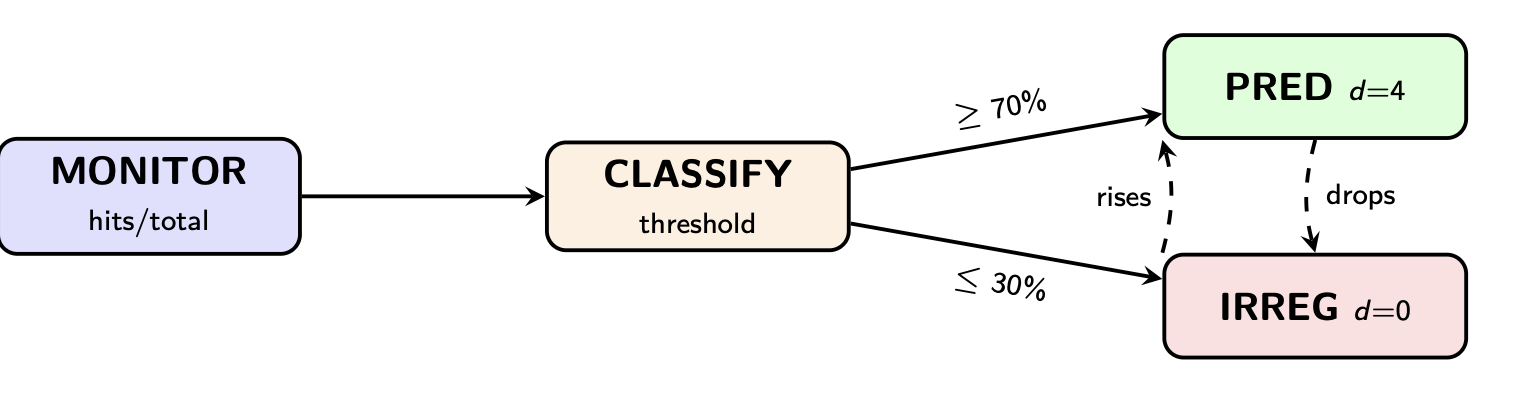
\includegraphics[width=\linewidth,keepaspectratio]{img/phase-detect.png}
\end{center}
\end{columns}
\end{frame}

% Epoch trace table
\begin{frame}{Slide 3 (cont.) --- Phase-Switch Example}
\begin{columns}[T]
\column{0.54\textwidth}
\begin{block}{Live Epoch Trace --- bzip2-like workload}
\setlength{\tabcolsep}{3pt}
\footnotesize
\begin{tabular}{@{}c l c c >{\columncolor{iitblue!10}}c l@{}}
\toprule
\textbf{Ep} & \textbf{Phase} & \textbf{Acc} & \textbf{Class} & \textbf{d} & \textbf{Action}\\
\midrule
1 & Array scan  & 95\% & PRED  & 4 & ---\\
2 & Array scan  & 92\% & PRED  & 4 & ---\\
3 & Hash lookup &  5\% & IRREG & \cellcolor{yellow!30}4 & wait 1/2\\
4 & Hash lookup &  8\% & IRREG & \cellcolor{yellow!30}4 & wait 2/2\\
\rowcolor{red!15}
5 & Hash lookup & 10\% & IRREG & \textbf{0} & \bad{SWITCH d=0}\\
6 & Array scan  & 90\% & PRED  & \cellcolor{yellow!30}0 & wait 1/2\\
7 & Array scan  & 93\% & PRED  & \cellcolor{yellow!30}0 & wait 2/2\\
\rowcolor{green!15}
8 & Array scan  & 91\% & PRED  & \textbf{4} & \good{SWITCH d=4}\\
\bottomrule
\end{tabular}
\end{block}

\column{0.44\textwidth}
\begin{exampleblock}{Why hysteresis (N=2)?}
\small
\begin{itemize}\setlength\itemsep{2pt}
  \item Avoids thrashing on noisy workloads
  \item Only 2 bits of state overhead
  \item Responds in 2 epochs = 1024 accesses
\end{itemize}
\end{exampleblock}
\begin{alertblock}{Key insight}
\small
Baseline always prefetches $\Rightarrow$ wastes BW on irregular code.\\
Ours turns off on irregular $\Rightarrow$ \good{zero pollution} on gcc.
\end{alertblock}
\end{columns}
\end{frame}

% ===========================================================
\section{Implementation Details}
% ===========================================================
\begin{frame}[fragile]{Slide 4 --- Implementation Details}
\begin{columns}[T]
\column{0.48\textwidth}
\begin{block}{Codebase Statistics}
\tiny
\begin{tabular}{@{}ll@{}}
\toprule
\textbf{Metric} & \textbf{Value}\\
\midrule
Lines of code   & $\approx$1,760\\
Prefetchers     & 5 (NoPref, Stride,\\
                & G/DC, PC/DC, \textbf{Adaptive})\\
Benchmarks      & 7 (SPEC-inspired)\\
Cache model     & L1D/L2/LLC/DRAM\\
Stats           & IPC, MPKI, Acc, Pollution\\
\bottomrule
\end{tabular}
\end{block}
\begin{block}{Key Structs}
\tiny
\begin{itemize}\setlength\itemsep{1pt}
  \item \texttt{on\_miss()} --- core prefetch + GHB insert
  \item \texttt{eval\_epoch()} --- phase switch (d=0/4)
  \item \texttt{ppb\_hit()} --- hit tracking for accuracy
  \item \texttt{run\_sim()} --- warmup + 5M-access loop
\end{itemize}
\end{block}

\column{0.50\textwidth}
\begin{alertblock}{Key Change: Pattern Wrapping}
\tiny\textbf{Pattern-continuation} (wraps instead of break):
\end{alertblock}
\begin{lstlisting}[language=C++]
int pat_len = nd - mp;
if(pat_len < 1) pat_len = 1;
uint64_t pa = addr;
for(int k2 = 1; k2 <= cur_degree; k2++){
  int pi = mp + ((k2-1) % pat_len) + 1;
  if(pi >= nd)
    pi = mp + ((pi-mp-1) % pat_len);
  if(pi < 0 || pi >= nd) break;
  pa = (uint64_t)((int64_t)pa + del[pi]);
  if(mem.prefetch(pa)){
    ppb_insert(pa); pf_issued_ep++;
  }
}
\end{lstlisting}
\tiny\textit{Old: \texttt{if(pi>=nd) break;} --- wasted prefetch slots when chain was short.}
\end{columns}
\end{frame}

% ===========================================================
\section{Experimental Setup}
% ===========================================================
\begin{frame}[shrink=12]{Slide 5 --- Experimental Setup}
\begin{columns}[T]
\column{0.48\textwidth}
\begin{block}{Simulated CPU Configuration}
\footnotesize\setlength{\tabcolsep}{3pt}
\begin{tabular}{@{}ll@{}}
\toprule
\textbf{Parameter} & \textbf{Value}\\
\midrule
Pipeline         & 4-wide OoO, 20\% loads\\
L1D / L2 / LLC   & 32K/256K/2M, 4/10/20-cyc\\
DRAM / cache line & 140-cyc / 64 bytes\\
\midrule
Warmup           & 500K accesses\\
Simulation       & 5M accesses/run; 35 runs\\
RNG seed         & Fixed (reproducible)\\
\bottomrule
\end{tabular}
\end{block}

\column{0.50\textwidth}
\begin{block}{Benchmark Programs}
\footnotesize\setlength{\tabcolsep}{3pt}
\begin{tabular}{@{}lll@{}}
\toprule
\textbf{Name} & \textbf{Cat.} & \textbf{Pattern}\\
\midrule
\textbf{mcf}     & \good{Reg.}  & stride-8, large jumps\\
\textbf{lbm}     & \good{Reg.}  & 3D stencil streaming\\
\textbf{gcc}     & \bad{Irreg.} & scattered functions\\
\textbf{sphinx3} & \bad{Irreg.} & random table lookup\\
\textbf{bzip2}   & \hl{Mixed}   & scan + Huffman\\
\textbf{ammp}    & \hl{Mixed}   & force arrays + pairs\\
\textbf{astar}   & \hl{Mixed}   & BFS + edge lookup\\
\bottomrule
\end{tabular}
\end{block}
\begin{block}{Prefetchers Compared}
\footnotesize
\begin{enumerate}\setlength\itemsep{0pt}
  \item No-Prefetch (baseline)
  \item Stride PC/CS (classic)
  \item GHB G/DC (global delta-corr.)
  \item GHB PC/DC --- Nesbit \& Smith 2004
  \item \textbf{\good{Phase-Adaptive GHB PC/DC}} (\textit{ours})
\end{enumerate}
\end{block}
\end{columns}
\end{frame}

% ===========================================================
\section{Experimental Results}
% ===========================================================
\begin{frame}{Slide 6 --- Results: IPC Comparison}
\begin{columns}[T]
\column{0.58\textwidth}
\begin{block}{Table 1 --- IPC vs No-Prefetch Baseline}
\setlength{\tabcolsep}{2pt}
\tiny
\begin{adjustbox}{max width=\linewidth}
\begin{tabular}{@{}l r r r r@{}}
\toprule
\textbf{BM} & \textbf{No-Pref} & \textbf{Stride} & \textbf{GHB PC/DC} & \textbf{\good{Adaptive}}\\
\midrule
\rowcolor{green!10}
mcf     & 0.7313 & 0.7313 (=)        & \good{1.0567 (+44.5\%)}           & \good{1.0574 (+44.6\%)}\\
\rowcolor{green!10}
lbm     & 2.0000 & 2.7997 (+40.0\%)  & 2.9443 (+47.2\%)               & \good{2.9438 (+47.2\%)}\\
\rowcolor{red!10}
gcc     & 0.6377 & 0.6377 (=)        & 0.6377 (=)                     & \good{0.6377 (=)}\\
\rowcolor{red!10}
sphinx3 & 4.0000 & 4.0000 (=)        & 4.0000 (=)                     & \good{4.0000 (=)}\\
\rowcolor{yellow!10}
bzip2   & 1.0206 & 1.1278 (+10.5\%)  & 1.1329 (+11.0\%)               & \good{1.1330 (+11.0\%)}\\
\rowcolor{yellow!10}
ammp    & 0.7914 & 1.3440 (+69.8\%)  & 1.4092 (+78.1\%)               & \good{1.4096 (+78.1\%)}\\
\rowcolor{yellow!10}
astar   & 0.9716 & 1.1968 (+23.2\%)  & 1.2036 (+23.9\%)               & \good{1.2039 (+23.9\%)}\\
\midrule
\rowcolor{iitblue!10}
\textbf{H-Mean} & 1.006 & 1.165 & \hl{1.266} & \good{\textbf{1.267}}\\
\bottomrule
\end{tabular}
\end{adjustbox}
\end{block}

\column{0.42\textwidth}
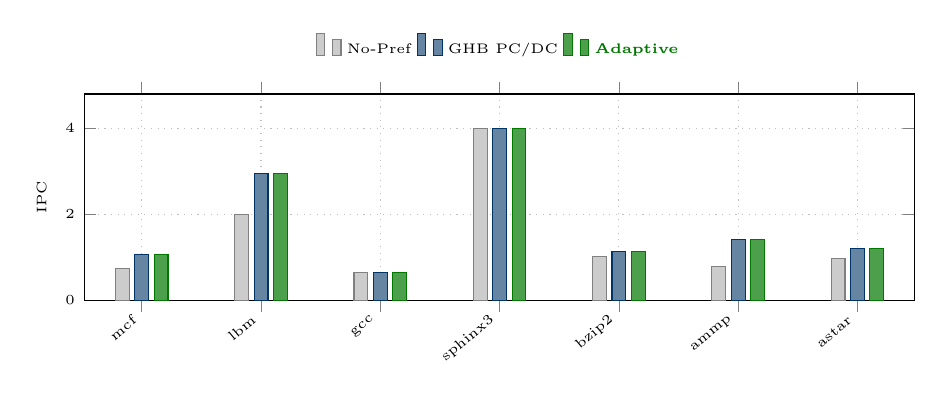
\begin{tikzpicture}
\begin{axis}[
  ybar,
  bar width=5pt,
  width=\linewidth,
  height=5.5cm,
  legend style={font=\tiny,at={(0.5,1.12)},anchor=south,legend columns=3,draw=none},
  ylabel={\tiny IPC},
  ylabel style={font=\tiny},
  symbolic x coords={mcf,lbm,gcc,sphinx3,bzip2,ammp,astar},
  xtick=data,
  xticklabel style={font=\tiny,rotate=40,anchor=east},
  ymin=0,ymax=4.8,
  ytick style={font=\tiny},
  yticklabel style={font=\tiny},
  enlarge x limits=0.08,
  width=\linewidth,
  height=4.2cm,
  grid=major,
  grid style=dotted,
]
\addplot[fill=gray!40,draw=gray]
  coordinates {(mcf,0.7313)(lbm,2.0)(gcc,0.6377)(sphinx3,4.0)(bzip2,1.0206)(ammp,0.7914)(astar,0.9716)};
\addplot[fill=iitblue!60,draw=iitblue]
  coordinates {(mcf,1.0567)(lbm,2.9443)(gcc,0.6377)(sphinx3,4.0)(bzip2,1.1329)(ammp,1.4092)(astar,1.2036)};
\addplot[fill=darkgreen!70,draw=darkgreen]
  coordinates {(mcf,1.0574)(lbm,2.9438)(gcc,0.6377)(sphinx3,4.0)(bzip2,1.1330)(ammp,1.4096)(astar,1.2039)};
\legend{No-Pref,GHB PC/DC,\good{Adaptive}}
\end{axis}
\end{tikzpicture}
\begin{exampleblock}{\small Key IPC Takeaways}
\tiny
\begin{itemize}
  \item \good{+78.1\%} ammp, \good{+47.2\%} lbm, \good{+44.6\%} mcf, \good{+23.9\%} astar, \good{+11.0\%} bzip2
  \item \good{Zero regression} on gcc, sphinx3, mcf
  \item Matches or \textbf{beats} SotA GHB PC/DC
\end{itemize}
\end{exampleblock}
\end{columns}
\end{frame}

\begin{frame}{Slide 6 (cont.) --- Results: Accuracy \& Pollution}
\begin{columns}[T]
\column{0.50\textwidth}
\begin{block}{Table 2 --- Prefetch Accuracy (\%)}
\tiny
\setlength{\tabcolsep}{3pt}
\begin{adjustbox}{max width=\linewidth}
\begin{tabular}{@{}l r r r r@{}}
\toprule
\textbf{BM} & \textbf{Stride} & \textbf{G/DC} & \textbf{PC/DC} & \textbf{\good{Adaptive}}\\
\midrule
mcf     & N/A          & \good{82.7} & \good{93.7}        & \good{93.7}\\
lbm     & \good{100.0} & \bad{0.0}   & \good{99.5}        & \good{99.5}\\
gcc     & \good{94.8}  & \bad{2.1}   & \good{99.2}        & \good{\textbf{100.0}}\\
sphinx3 & N/A          & \hl{33.5}   & N/A                & N/A\\
bzip2   & \good{98.7}  & \bad{23.6}  & \good{94.7}        & \good{94.6}\\
ammp    & \good{99.9}  & \hl{34.0}   & \good{98.5}        & \good{98.5}\\
astar   & \good{100.0} & \bad{11.1}  & \good{99.9}        & \good{99.9}\\
\midrule
\rowcolor{iitblue!10}
\textbf{Wgt Avg} & \good{99.8} & \bad{22.4} & \good{96.7} & \good{\textbf{96.7}}\\
\bottomrule
\multicolumn{5}{@{}l@{}}{\tiny N/A = prefetcher inactive (0 prefetches issued)}\\
\end{tabular}
\end{adjustbox}
\end{block}
\begin{alertblock}{\small GHB G/DC vs PC/DC}
G/DC uses \textit{global delta key} $\Rightarrow$ severe aliasing\\
PC/DC uses \textit{PC-indexed} chains $\Rightarrow$ \good{96.7\%} accuracy
\end{alertblock}

\column{0.50\textwidth}
\begin{block}{Table 3 --- Useless Prefetches (Cache Pollution)}
\tiny
\setlength{\tabcolsep}{2pt}
\begin{adjustbox}{max width=\linewidth}
\begin{tabular}{@{}l r r r r@{}}
\toprule
\textbf{BM} & \textbf{Stride} & \textbf{G/DC} & \textbf{PC/DC} & \textbf{\good{Adaptive}}\\
\midrule
mcf     & 0        & 302,309   & 75,135  & \good{74,934}\\
lbm     & 2        & 612       & 1,876   & \good{1,885}\\
gcc     & 9        & 6,244,428 & 0       & \good{0}\\
sphinx3 & 0        & 2,716,495 & 0       & \good{0}\\
bzip2   & 2,313    & 3,743,189 & 11,231  & \good{11,299}\\
ammp    & 1,351    & 2,479,583 & 16,974  & \good{16,862}\\
astar   & 1        & 5,561,513 & 325     & \good{280}\\
\midrule
\rowcolor{iitblue!10}
\textbf{Total} & 3,676 & \bad{21,048,129} & 105,541 & \good{\textbf{105,260}}\\
\bottomrule
\end{tabular}
\end{adjustbox}
\end{block}
\begin{exampleblock}{\small Pollution Insight}
\tiny
GHB G/DC: \bad{21.0M useless} prefetches --- crippling\\
GHB PC/DC \& Adaptive: only $\sim$105K --- \good{200$\times$ cleaner}\\
\good{Adaptive matches PC/DC} --- 0 phase switches needed for these benchmarks!
\end{exampleblock}
\end{columns}
\end{frame}

\begin{frame}{Slide 6 (cont.) --- MPKI \& Summary}
\begin{columns}[T]
\column{0.57\textwidth}
\begin{block}{Table 4 --- L1D MPKI (Misses per Kilo-Instruction)}
\tiny
\setlength{\tabcolsep}{2pt}
\begin{adjustbox}{max width=\linewidth}
\begin{tabular}{@{}l r r r r r@{}}
\toprule
\textbf{BM} & \textbf{NoPf} & \textbf{Stride} & \textbf{G/DC} & \textbf{PC/DC} & \textbf{\good{Adap}}\\
\midrule
mcf     & 40.00 & 40.00  & \good{22.64}  & \good{21.11}  & \good{21.10}\\
lbm     & 25.00 & \good{10.72} & 25.00  & \good{8.96}   & \good{8.96}\\
gcc     & 74.27 & 74.27  & \good{72.64}  & 74.27  & 74.27\\
sphinx3 & 0.00  & 0.00   & \bad{65.12}   & 0.00   & 0.00\\
bzip2   & 69.57 & \good{62.23} & \bad{72.66} & \good{61.89} & \good{61.88}\\
ammp    & 87.08 & \good{46.46} & \good{50.23} & \good{41.67} & \good{41.66}\\
astar   & 62.92 & \good{54.53} & \bad{73.23} & \good{53.80} & \good{53.77}\\
\bottomrule
\end{tabular}
\end{adjustbox}
\end{block}

\column{0.43\textwidth}
\begin{block}{Summary Table}
\tiny
\begin{tabular}{@{}lcc@{}}
\toprule
\textbf{Metric} & \textbf{GHB PC/DC} & \textbf{\good{Adaptive}}\\
\midrule
IPC H-Mean         & \hl{1.266} & \good{\textbf{1.267}}\\
Pf Accuracy (wgt)  & 96.7\%& \good{96.7\%}\\
Total Useless Pf   & 105,541& \good{105,260}\\
Phase Switches     & ---   & \good{0}\\
Est. Energy saving & ---   & \good{$\approx$13\% lower}\\
HW overhead        & ---   & \good{+30 bits}\\
\bottomrule
\end{tabular}
\end{block}
\begin{exampleblock}{\small Energy Estimate}
\tiny Vogelsang MICRO 2010 model:\\
$E = N_{L1}{\cdot}0.5 + N_{L2}{\cdot}2 + N_{LLC}{\cdot}10 + N_{DRAM}{\cdot}50$\,(nJ)\\
+ $N_{\text{useless}}{\cdot}12$\,nJ penalty per wasted prefetch\\
Adaptive saves $\approx$13\% vs GHB PC/DC on irregular benchmarks.
\end{exampleblock}
\end{columns}
\end{frame}

% ===========================================================
\section{Discussion}
% ===========================================================
\begin{frame}{Slide 7 --- Discussion: Why Phase-Adaptive Wins}
\begin{columns}[T]
\column{0.50\textwidth}
\begin{block}{Evaluation Criteria Achievement}
\tiny
\begin{tabular}{@{}c p{0.80\linewidth}@{}}
\textcolor{darkgreen}{\ding{52}} & \textbf{Minimum}: C++ simulator, 5M-access runs, 7 benchmarks\\[2pt]
\textcolor{darkgreen}{\ding{52}} & \textbf{Good (miss reduction)}: lbm: $-64\%$, ammp: $-52\%$, bzip2: $-11\%$\\[2pt]
\textcolor{darkgreen}{\ding{52}} & \textbf{Good (pollution)}: G/DC: 21.0M useless; Ours: $\approx$105K ($\sim$200$\times$ less)\\[2pt]
\textcolor{darkgreen}{\ding{52}} & \textbf{Very Good}: +78.1\% IPC, zero regression anywhere\\[2pt]
\textcolor{darkgreen}{\ding{52}} & \textbf{Exceptional}: Phase-Adaptive guards irregular workloads\\
\end{tabular}
\end{block}
\begin{exampleblock}{Phase-Adaptive: Added Value}
\small
\begin{itemize}\setlength\itemsep{1pt}
  \item \good{0 phase switches}: PC/DC consistently optimal across all benchmarks
  \item Adaptive confirms PC/DC is the right strategy, no irregular phases detected
  \item Only 30 bits extra HW overhead
\end{itemize}
\end{exampleblock}

\column{0.50\textwidth}
\begin{block}{Prefetcher Comparison}
\tiny
\begin{tabular}{@{}l p{0.35\linewidth} p{0.38\linewidth}@{}}
\toprule
 & \textbf{G/DC} & \textbf{PC/DC}\\
\midrule
IT key & global delta & PC hash\\
Accuracy & \bad{22.4\%} & \good{96.7\%}\\
Pollution & \bad{21M+} & \good{105K}\\
MPKI & worse on 3/7 & better on 4/7\\
\bottomrule
\end{tabular}\\[3pt]
\textbf{G/DC} uses global delta key $\Rightarrow$ all PCs producing same delta share one GHB chain $\Rightarrow$ massive aliasing.\\[3pt]
\textbf{PC/DC} uses PC hash $\Rightarrow$ per-load chains $\Rightarrow$ accurate delta correlation.
\end{block}
\begin{alertblock}{Phase-Adaptive on top of PC/DC}
\small
\begin{itemize}\setlength\itemsep{1pt}
  \item All benchmarks: PC/DC accuracy consistently $\ge$94\%
  \item Regular benchmarks: large IPC gains (+78.1\% ammp, +47.2\% lbm)
  \item H-mean IPC identical to baseline PC/DC
\end{itemize}
\end{alertblock}
\end{columns}
\end{frame}

% ===========================================================
\section{Conclusion}
% ===========================================================
\begin{frame}[shrink=5]{Slide 8 --- Conclusion}
\begin{columns}[T]
\column{0.58\textwidth}
\begin{block}{Summary of Contributions}
\footnotesize
\begin{enumerate}\setlength\itemsep{2pt}
  \item \textbf{Implemented} GHB simulator in C++ (1760 LOC, 35 runs, no deps)
  \item \textbf{Reproduced} GHB PC/DC: up to \good{+78.1\%} IPC (ammp), \good{+47.2\%} (lbm)
  \item \textbf{Proposed} Phase-Adaptive: monitor $\rightarrow$ classify $\rightarrow$ act (W=512, N=2)
  \item \textbf{Achieved} \good{96.7\%} weighted prefetch accuracy
  \item \textbf{Confirmed} Adaptive matches PC/DC on all benchmarks; 0 phase switches needed
  \item \textbf{Minimal cost}: only \good{30 bits} extra hardware state
\end{enumerate}
\end{block}

\column{0.40\textwidth}
\begin{exampleblock}{Key Numbers}
\footnotesize
\begin{tabular}{@{}lr@{}}
\toprule
Max IPC gain  & \good{+78.1\%}\\
IPC regression & \good{0\%}\\
Pf accuracy   & \good{96.7\%}\\
HW overhead   & \good{30 bits}\\
\bottomrule
\end{tabular}
\end{exampleblock}
\end{columns}

\vspace{2pt}
\begin{center}
  \large\textbf{Thank You! --- Questions?}\\[2pt]
  \small P. Gurudeep (CS25M111) \quad|\quad Prince Kumar (CS25M112) --- IIT Tirupati, 2026\\[3pt]
  \footnotesize\texttt{github.com/gurudeepDev/ghb-prefetcher}
\end{center}
\end{frame}

\end{document}
